\documentclass{beamer}
\usetheme{AnnArbor}
\usecolortheme{wolverine}
\usepackage{graphicx}
\usepackage{booktabs}
\usepackage[english]{babel}
\usepackage[backend=biber,style=numeric, citestyle=ieee]{biblatex}
\addbibresource{./main.bib}

\title[Image Fusion using GAN]{Fusion of Multi-spectral and Hyper-spectral Data for classification.}
\author[Advaith C A]{Advaith C A,\\MTech, PRSD.\\Guide: Mr Vinay Kumar}
\date{\today}

\begin{document}
\begin{frame}
    \maketitle
\end{frame}
\begin{frame}{Overview}
    \hfill
    \parbox[t]{.89\textwidth}{
      \begin{minipage}[c][0.6\textheight]{\textwidth}
      \tableofcontents
      \end{minipage}
    }
\end{frame}
\section{Introduction}
\begin{frame}{Introduction}
    \begin{itemize}
        \item \textbf{Fusion in Remote Sensing} - Improve the spectral resolution without loss in spatial resolution.
        \item \textbf{Conventional techniques for Fusion} include IHS image fusion, Brovey transform image fusion, Principal Component Analysis image fusion, Wavelet image fusion etc.
        \item \textbf{Generative Adversarial Network} is a type of Neural Network that has two components - a Generator and a Discriminator.
        \item GAN can be used in RS fusion. GAN has been used for Neural Style transfer in which the style data of one image is transferred to another.
        \item GAN models opposing relationships, such relationships are present widely in remote sensing.
    \end{itemize}
\end{frame}

\section{Image Fusion}
\begin{frame}{Image Fusion}
    \begin{enumerate}
        \item Combines properties of multiple images to produce outputs that have the best of both (all) worlds.
        \item Fused output usually provides more information than any of the images taken one at a time.
    \end{enumerate}
\end{frame}
\begin{frame}{Why image fusion?}
    \begin{enumerate}
        \item Improved spatial and spectral resolution.
        \item Wider temporal coverage.
        \item Better performance in tasks such as classification.
        \item Good fusion technique has the following characteristics: high computational efficiency, better spatial resolution, reduced color distortion.
    \end{enumerate}
\end{frame}
\section{Generative Adversarial Networks}
\begin{frame}{Generative Adversarial Networks}
    \begin{itemize}
        \item GAN was proposed by Goodfellow et al. \cite{Goodfellow2020}
        \item \textit{GAN}s are a kind of Neural Networks that consist of two neural networks - one acting as a discriminator, another as a generator.
        \item The \textit{generator} learns the data distribution, and tries to generate the distribution.
        \item The \textit{discriminator} tries to predict whether the generated distribution is the data distribution or the model distribution.
    \end{itemize}
\end{frame}
\begin{frame}{Generative Adversarial Networks Contd..}
    \begin{figure}
        \centering
        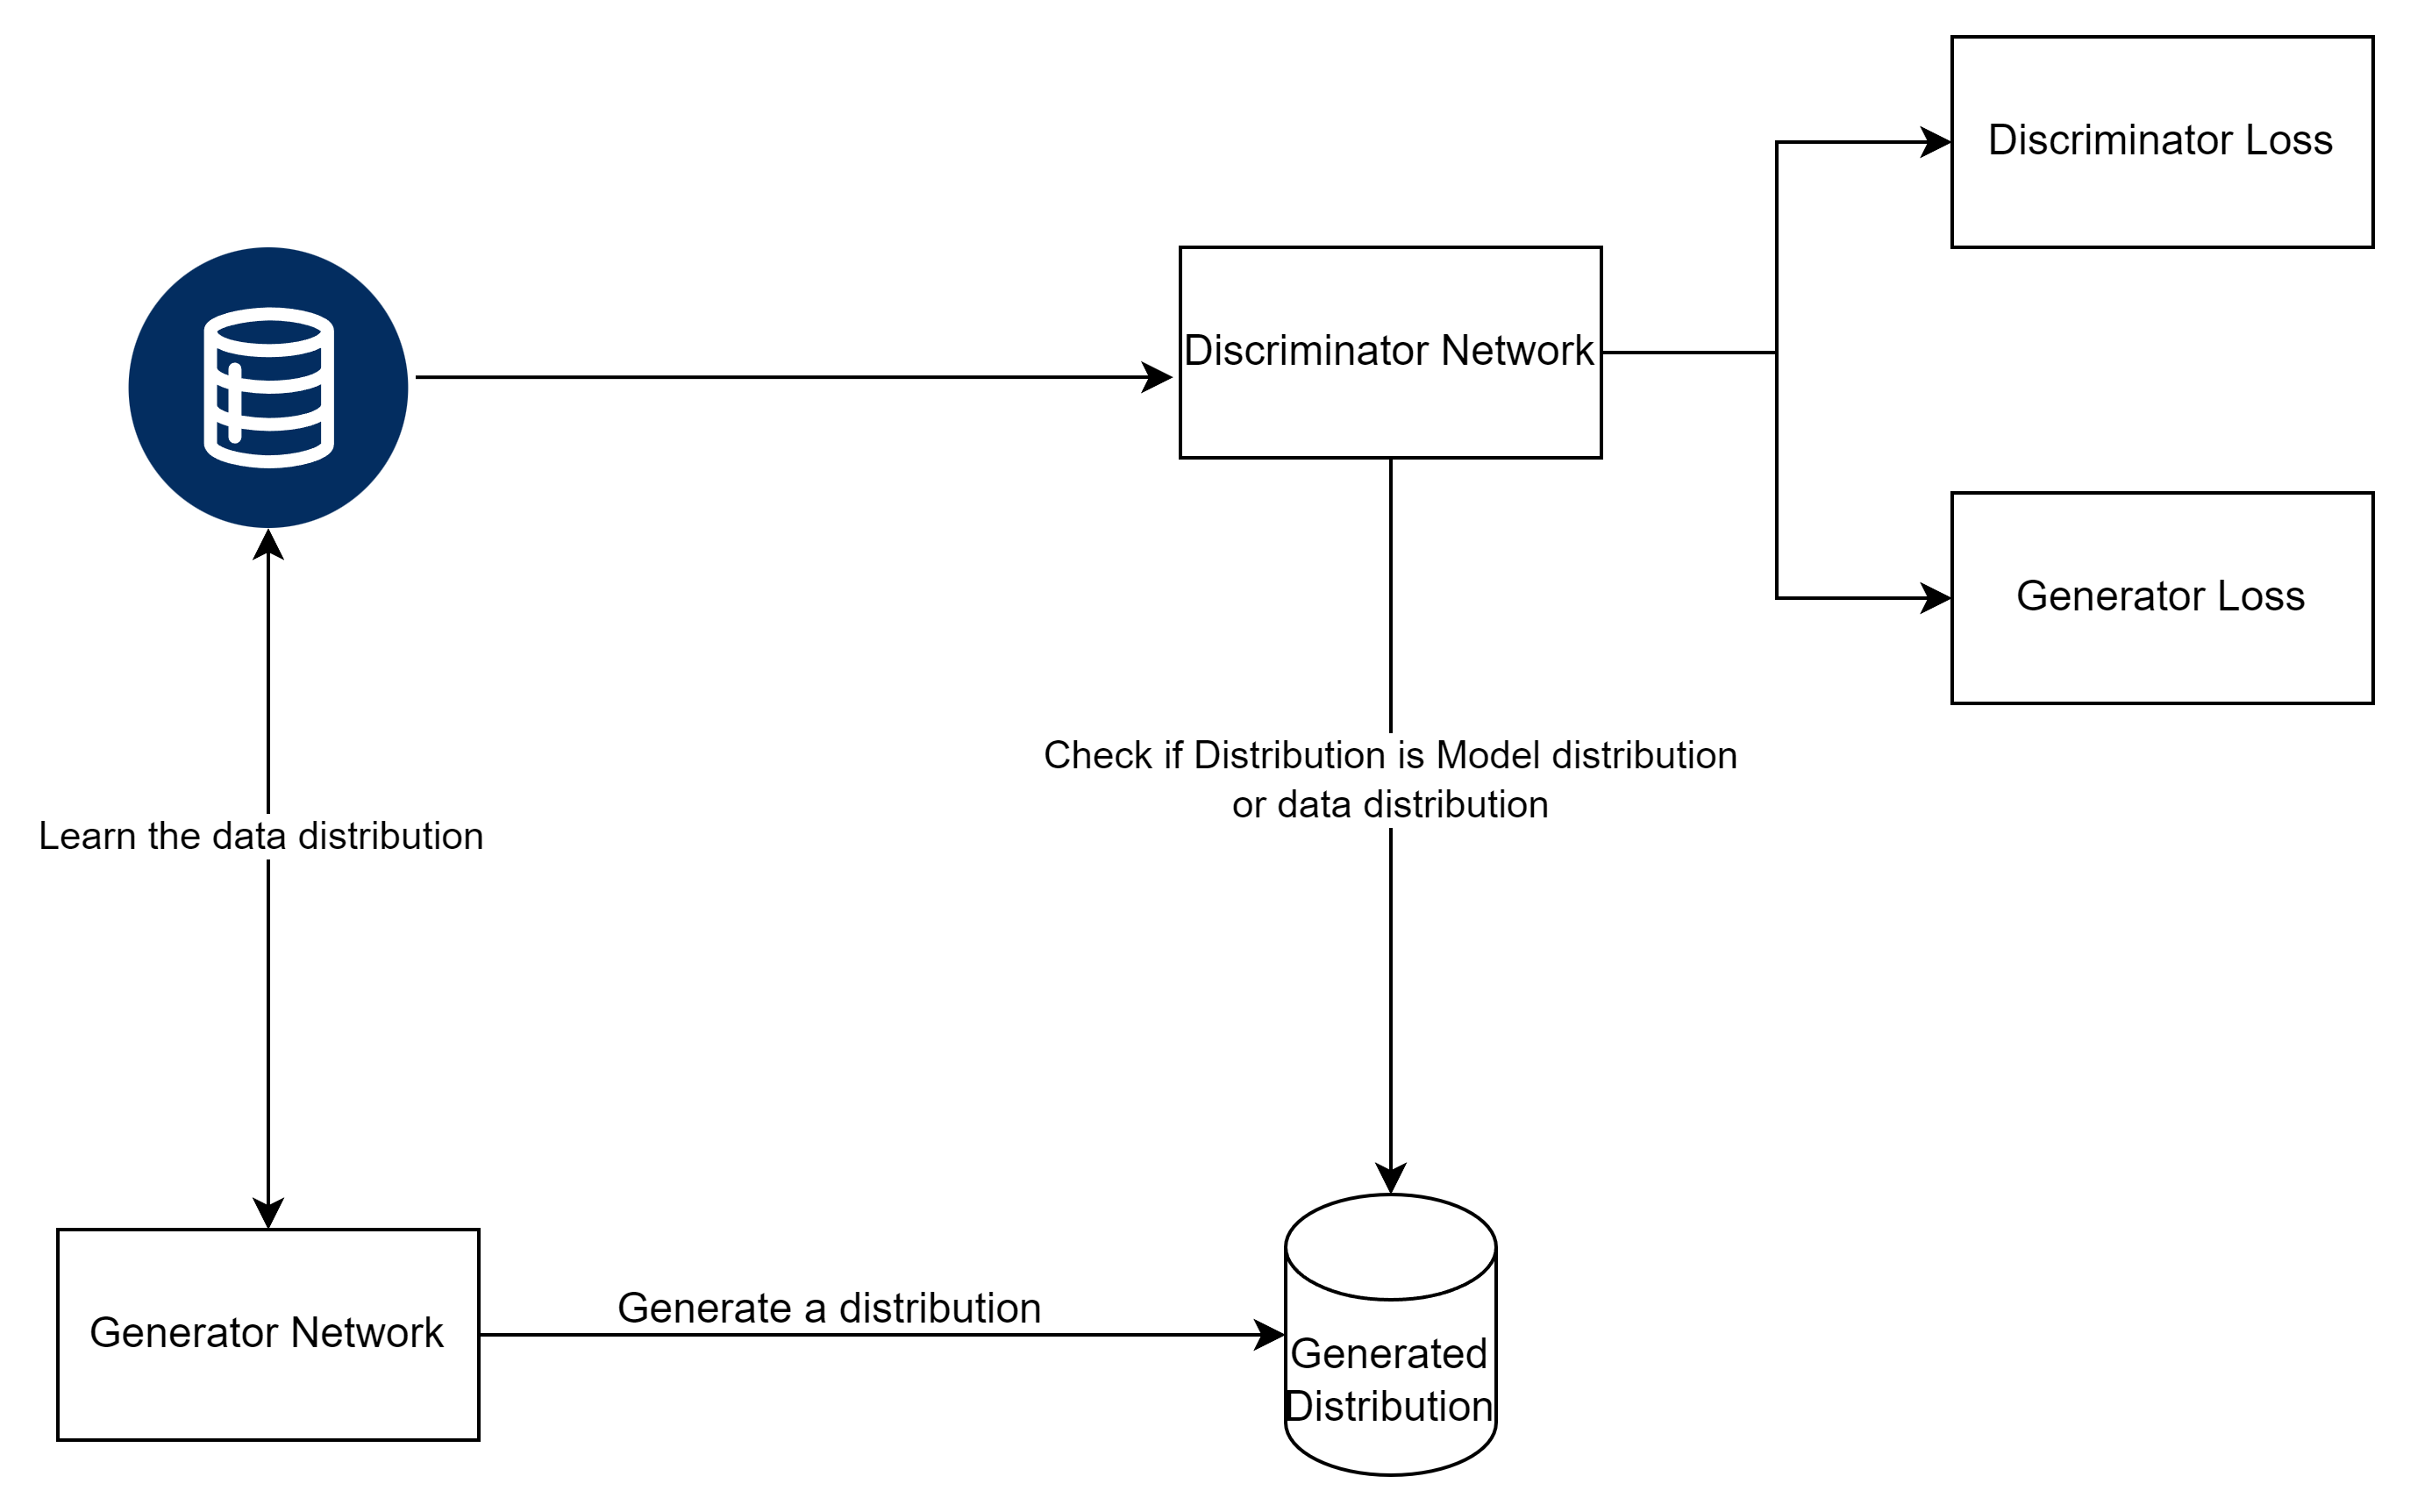
\includegraphics[width=0.7\textwidth]{../images/GAN.png}
        \caption{How the GAN Works}
        \label{fig:fig-1}
    \end{figure}
\end{frame}
\section{Image fusion using GAN}
\begin{frame}{Image fusion using GAN}
    \begin{itemize}
        \item For remote sensing data, raw GAN is not used; specialized GANs such as Unmixing-based Multi-attention GAN \cite{Su2023}, QIS-GAN \cite{Zhu2023}, SwinGAN \cite{Zhu2023a}, Physics-based GAN \cite{Xiao2021} are some State of the art techniques.
        \item There has not been much work done in the domain of Multispectral-hyperspectral spatial-spectral image fusion using GAN other than the papers mentioned before.
    \end{itemize}
\end{frame}
\begin{frame}{Image fusion using GAN contd...}
    \begin{itemize}
        \item The state of the art techniques like QIS-GAN, Unmixing-based GAN, SwinGAN were designed and trained on systems that had upwards of 64 GB RAM, and with GPU support (thousands of CUDA cores).
        \item What I will do:
        \begin{itemize}
            \item Try running vanilla GAN for image fusion (with required modifications)
            \item Once successful, implement QIS-GAN as it is lightweight.
        \end{itemize}
    \end{itemize}
\end{frame}
\section{Data}
\begin{frame}{Data}
    \begin{figure}
        \centering
        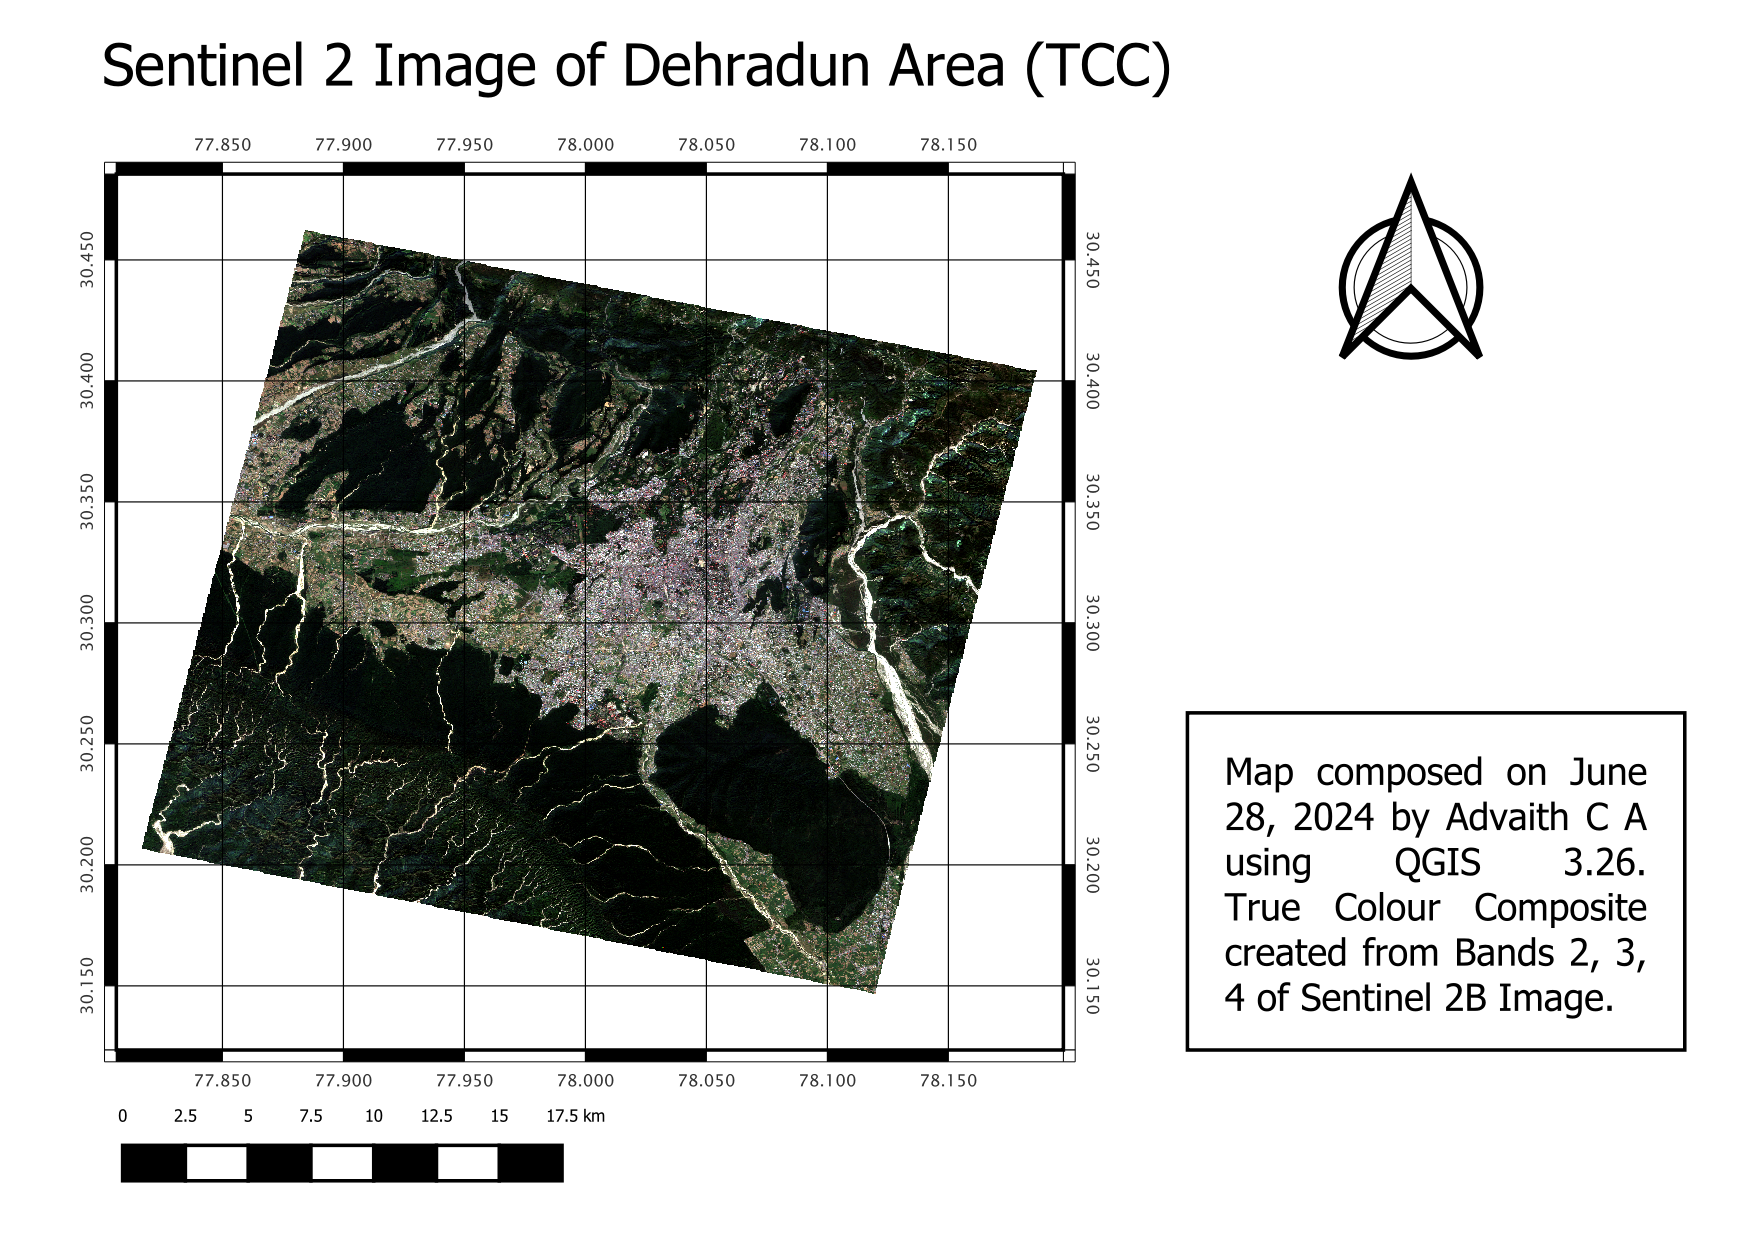
\includegraphics[width=0.75\textwidth]{../images/map_s2.png}
        \caption{The sentinel 2 image of Dehradun area}
        \label{fig:fig-2}
    \end{figure}
\end{frame}
\begin{frame}{Data}
    \begin{figure}
        \centering
        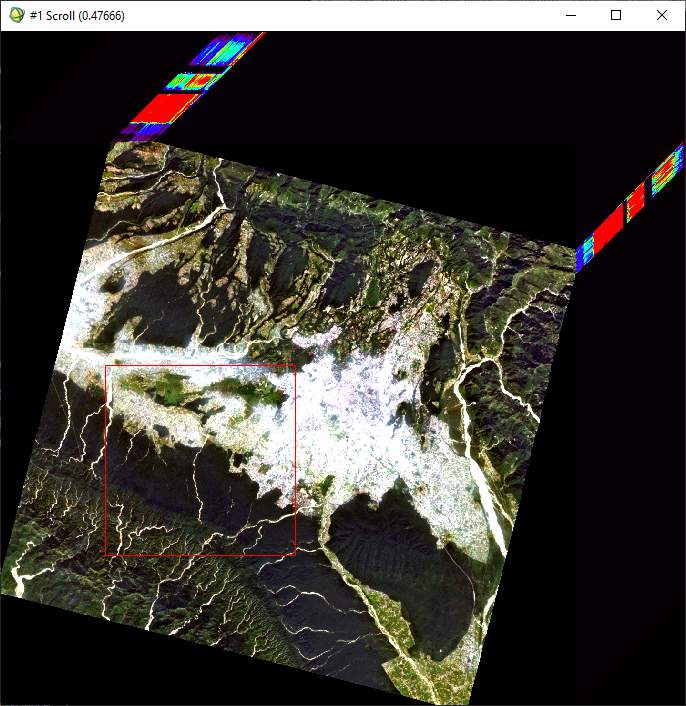
\includegraphics[width=0.5\linewidth]{../images/hyper.png}
        \caption{Screenshot of hyperspectral data of the same area, visualized as hypercube in ENVI class 5.0}
        \label{fig:fig-3}
    \end{figure}
\end{frame}
\section{Comparison}
\begin{frame}{GAN vs Conventional}
    \begin{table}
        \centering
        \begin{tabular}{|| p{5cm} | p{5cm} ||} 
             \hline
             \textbf{Generative Adversarial Networks} & \textbf{Conventional} \\ [0.5ex] 
             \hline\hline
             Can preserve spatial and spectral properties & There are chances for degradation \\ 
             \hline
             Less susceptible to noise & Noise can ruin the process \\
             \hline
             Adapts to different data distributions & There is no real "adaptation" to the data \\
             \hline
        \end{tabular}
        \caption{Comparison of GAN and Conventional methods for fusion.}
        \label{table:tab-1}
    \end{table}
\end{frame}
\section{References}
\begin{frame}[allowframebreaks]{References}
        \printbibliography
\end{frame}
\end{document}
